\documentclass[11pt]{article}
\usepackage[margin=1in, top=15pt]{geometry}
\usepackage{amsmath, amssymb, xcolor, booktabs, graphicx, tikz}
\usetikzlibrary{graphs, graphs.standard, quotes}
\title{CS 225}
\author{Graph Theory}
\date{Fall 2020}

\begin{document}
\maketitle
\hrule

% \begin{center}\underline{\bf \large Definitions}\end{center}
\bigskip

{\bf Graph:} A graph $G$ is a nonempty set $V(G)$ of vertices,
and a set $E(G)$ of edges, where each edge is associated with a 
set of either one or two vertices, called the {\bf endpoints} 
of that edge. 

\bigskip
Here is a graph vith $V(G) = \{v_1, v_2\}$ and $E(G) = \{e_1\} = \{\{v_1, v_2\}\}$: 

\begin{center}
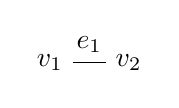
\begin{tikzpicture}
\graph {
    v1/$v_1$ -- ["$e_1$"] v2/$v_2$;
};
\end{tikzpicture}
\end{center}

\bigskip 
The {\bf edge to endpoint} function sends an edge to its set of endpoints. 
If we define an edge as the set of its endpoints (which we can do for simple 
graphs), this is pretty straightforward. 

\bigskip
An edge with just one endpoint is a loop (note that the loop drawn here is 
directed due to how my drawing program is working at the moment. Please 
ignore the arrow on the loop edge):
\begin{center}
    \begin{tikzpicture}
        \graph {
        v1/$v_1$ -- ["$e_1$", loop, swap] v1;
        };
    \end{tikzpicture}
\end{center}

Two or more {\it distinct} edges with the same set of endpoints are said 
to be {\bf parallel}:

\begin{center}
    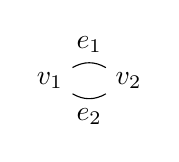
\begin{tikzpicture}
        \graph {
        v1/$v_1$ -- ["$e_1$", bend left] v2/$v_2$;
        v1/$v_1$ -- ["$e_2$", bend right, swap] v2/$v_2$;
        };
    \end{tikzpicture}
\end{center}

Two vertices connected by an edge are adjacent. In the picture below, $v_1$ 
and $v_2$ are adjacent vertices, and $v_2$ is adjacent to itself.

\begin{center}
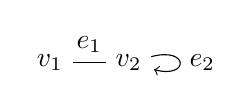
\begin{tikzpicture}
\graph {
    v1/$v_1$ -- ["$e_1$"] v2/$v_2$;
    v2 -- [loop right, "$e_2$"] v2;
};
\end{tikzpicture}
\end{center}

An edge is {\bf incident} on each of its endpoints, and two edges incident 
to the same endpoint are {\bf adjacent}. Below, edges $e_1$ and $e_2$ are 
adjacent since they share the endpoint $v_2$. 
\begin{center}
    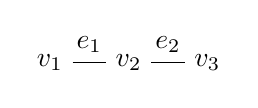
\begin{tikzpicture}
        \graph {
        v1/$v_1$ -- ["$e_1$"] v2/$v_2$ -- ["$e_2$"] v3/$v_3$;
        };
    \end{tikzpicture}
\end{center}

An isolated vertex:
\begin{center}
    \begin{tikzpicture}
        \graph {
          v1/$v_1$ -- v1/$v_1$;  
        };
    \end{tikzpicture}
\end{center}

\newpage
\newgeometry{top=1in}
A {\bf directed graph} has vertices and edges, but the edges are now ordered 
pairs. We can represent a directed graph as vertices and edges where the edges 
have arrows. Below is a graph with vertices $V(G) = \{v_1, v_2\}$ and directed 
edges $D(G) = \{e_1\} = \{(v_1, v_2)\}$. 

\begin{center}
    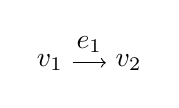
\begin{tikzpicture}
        \graph {
         v1/$v_1$ -> ["$e_1$"] v2/$v_2$;   
        };
    \end{tikzpicture}
\end{center}

If $G$ is a graph and $v$ is a vertex of $G$, then the {\bf degree} of $v$, 
$\deg(v)$ is the number of edges that are incident on $v$, with an edge that 
is a loop counted twice. Below $v_1$ has degree 1 and $v_2$ has degree 3:
\begin{center}
    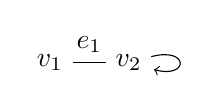
\begin{tikzpicture}
        \graph {
         v1/$v_1$ -- ["$e_1$"] v2/$v_2$ -- [loop right] v2;   
        };
    \end{tikzpicture}
\end{center}

The {\bf total degree} of a graph is the sum of degrees of all vertices of the 
graph. In the graph below, the total degree is 4. 
\begin{center}
    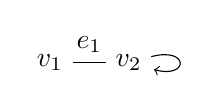
\begin{tikzpicture}
        \graph {
         v1/$v_1$ -- ["$e_1$"] v2/$v_2$ -- [loop right] v2;   
        };
    \end{tikzpicture}
\end{center}

\bigskip
{\bf Theorem 4.9.1: The handshake theorem} If $G$ is any graph then the sum of 
degrees of all the vertices of $G$ is equal to twice the number of edges of $G$. 

\bigskip
{\bf Corollary 4.9.2:} The total degree of a graph is even. 

\bigskip
{\bf Proposition 4.9.3:} In any graph there is an even number of vertices of 
odd degree. 

(if not then Corollary 4.9.2 would be false)

\bigskip
A {\bf simple} graph is a graph that does not have any loops or parallel edges. 

\bigskip
If $n$ is a positive integer, then a {\bf complete graph on $n$ vertices}, 
denoted $K_n$, is a simple graph with $n$ vertices and exactly one edge 
connecting each pair of distinct vertices. Below are $K_5$ and $K_{10}$:

\begin{center}
    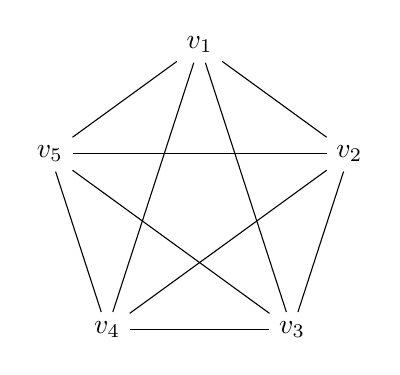
\begin{tikzpicture}
        \graph[clique, n=5, clockwise, radius=2cm, math nodes] {
            \foreach \i in {1, ..., 5}{
                v\i/v_\i,
            }
        };
    \end{tikzpicture}
\end{center}


\begin{center}
    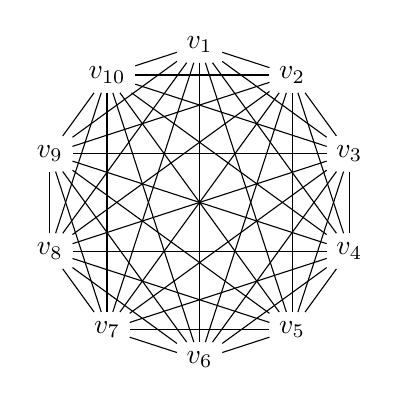
\begin{tikzpicture}
        \graph[clique, n=10, clockwise, radius=2cm, math nodes] {
            \foreach \i in {1, ..., 10}{
                v\i/v_{\i},
            }
        };
    \end{tikzpicture}
\end{center}

{\bf Example 4.9.9} $K_n$ has $\dfrac{n(n-1)}{2}$ edges. 

\bigskip
Let $m$ and $n$ be positive integers. A {\bf complete bipartite graph on $(m,n)$ 
vertices}, denoted $K_{m, n}$, is a simple graph whose vertices are divided 
into two distinct subsets, $V$ with $m$ vertices and $W$ with $n$ vertices, 
in such a way that 
\begin{enumerate}
    \item Every vertex of $K_{m,n}$ velongs to one of $V$ or $W$ but not both
    \item There is exactly one edge from each vertex of $V$ to each vertex of $W$
    \item There is no edge from any one vertex of $V$ to any other vertex of $V$. 
    \item There is no edge from any one vertex of $W$ to any other vertex of $W$. 
\end{enumerate}

$K_{3, 2}$ is shown below:

\begin{center}
    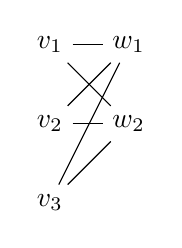
\begin{tikzpicture}
        \graph[ math nodes] {
        {\foreach \i in {1, ..., 3}{
            v\i / v_{\i},
        }} -- [complete bipartite]
        {\foreach \i in {1,2}{
            w\i / w_{\i},
        }}
        };
    \end{tikzpicture}
\end{center}
\end{document}